\documentclass[10pt]{article}
\usepackage[margin=15mm]{geometry}
\usepackage{graphicx,booktabs,hyperref}
\usepackage[strings]{underscore}
\setlength{\parindent}{0pt}\setlength{\parskip}{3pt}
\begin{document}
\section*{Complete-DLP smoke: K0 over GF($2^{13}$)}
Pricing correction: this supersedes the earlier report's pricing paragraph. Raw records and numerical bands are unchanged.

Report date 2026-10-25; session \texttt{ECBS1hd3bc41fb2eb2}.
All ten recorded answers verify and all ten deterministic replays reproduce.

Exact curve: \path{ICV1:f2m-13-752c6463:181:8012:0x1:-7:unk:r:515ee5696294}. Prime subgroup r=2003,
cofactor 4, generator (0x12b9,0x1bc4).
Two public known-answer one-target workloads, target seed 202610230101;
one round, no warmup, alternate order, per-child timeout 900 seconds.
Shared x86-64 host earns L0; elapsed times are diagnostic.

Arms: strong signed-Frobenius rho and its identical repeat; direct S4;
symmetric product-space S4 with degree-two closure; generic three-summand
MITM with negation folding. Every IC arm uses the same geometric factor
base, seed 17. Frozen complete parameters are in the session spec/plan.
The direct hybrid extraction has an input-degree floor, up to six.

\begin{center}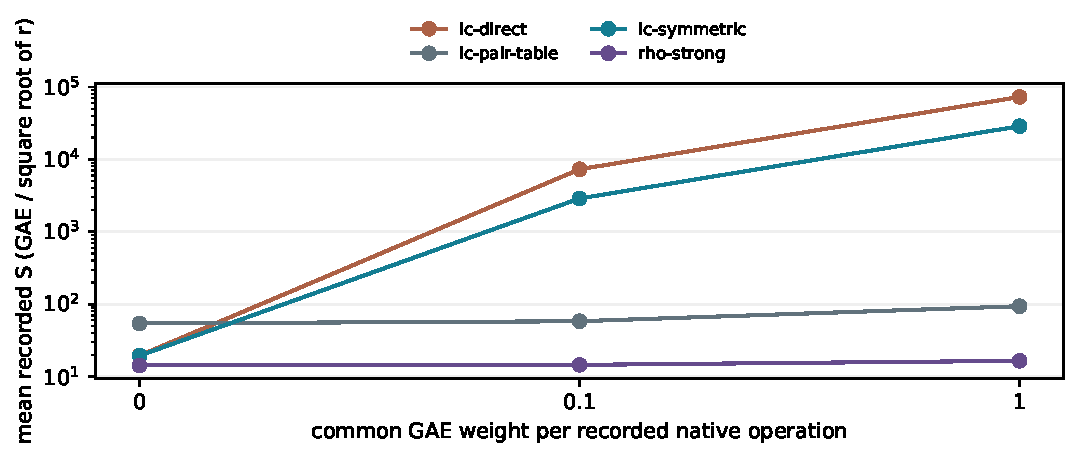
\includegraphics[width=.98\linewidth]{native-band.pdf}\end{center}

\begin{center}\begin{tabular}{lrl}\toprule
Arm & verified/planned & recorded S at weights 0 / 0.1 / 1\\\midrule
ic-direct & 2/2 & 19.57 / 7291 / 7.273e+04 \\
ic-pair-table & 2/2 & 54.28 / 58.25 / 93.89 \\
ic-symmetric & 2/2 & 19.47 / 2884 / 2.866e+04 \\
rho-strong & 2/2 & 14.33 / 14.55 / 16.55 \\
rho-strong-aa & 2/2 & 14.33 / 14.55 / 16.55 \\
\bottomrule\end{tabular}\end{center}

The graph quotes native ecbench band output, which re-prices recorded
group and native counters. It omits incompletely counted construction and
cubic splitting, and is not a complete-price comparison. No population
interval is claimed from two targets. The earlier report incorrectly said
raw S contains solver wall time. Actual completed n13/n23 solver charges
use pinned word rates. The measured n7 solver term is removed. Native
ic_campaign_pricing_audit reconstructs the available IC costs from integer
counts and fixed prices, matching the raw records. Raw S is a fixed-price
estimate of counted work, with the omissions above. The raw lower-bound flag does not mark these
omissions. Automated pair ranks do not repair missing costs or censored runs.

Source pushed through a5ff7036; the sealed records pin the actual binary.
The independent native audit reports 10 records,
10 verified, and 10 reproduced
replays, zero audit problems. Same-host replay checks correctness and
deterministic counts, not independent-host physical performance.

Raw sealed directory: \path{../../pipeline-runs/structured-n13-20261025-01/}.
Native replay: \path{../../pipeline-receipts/structured-n13-20261025-01.json};
native band: \path{../../pipeline-receipts/structured-n13-band.json}.
Plugin source: src/bin/ecbench/structured_s4.rs and structured_s4_math.rs.
All original failures remain recorded. No full IC gain or rho crossover
is promoted to the leaderboard or benchmark results table.

\end{document}
